\documentclass[conference]{IEEEtran}
\usepackage[utf8]{inputenc}
\usepackage[T1]{fontenc}
\usepackage{lmodern}
\pdfmapfile{+lm.map}
\usepackage{array,booktabs,graphicx,listings,url,balance}
\usepackage[hidelinks]{hyperref}
\renewcommand{\abstractname}{Resumen}
\renewcommand{\tablename}{Tabla}
\renewcommand{\figurename}{Fig.}
\renewcommand{\refname}{Referencias}
\renewcommand{\lstlistingname}{Código}
\lstset{basicstyle=\ttfamily\footnotesize,breaklines=true,columns=fullflexible,keepspaces=true,frame=single,captionpos=b}
\newcommand{\longidentifier}[1]{\texttt{#1}}
\setlength{\emergencystretch}{2em}
\begin{document}
\title{FitPulse: historias, modelo de datos y backend REST}
\author{\IEEEauthorblockN{Laura Triana}}
\maketitle
\begin{abstract}
Se presentan las historias de usuario, el modelo de siete tablas y las decisiones REST, de arquitectura e implementación del backend de FitPulse. La trazabilidad relaciona los requisitos con la persistencia y las solicitudes de prueba. Estos bloques están preparados para integrarse en el informe general; su compilación independiente permite revisar su coherencia sin atribuirse las secciones de otras integrantes.
\end{abstract}
\section{Historias de usuario}\label{sec:historias-laura}
Las historias expresan el rol, la acción y el beneficio esperado. Se conservan los códigos CO y AO para relacionarlas con los requerimientos y con las operaciones de la API. Las Tablas~\ref{tab:historias-clientes-laura} y~\ref{tab:historias-admin-laura} reúnen las 18 historias.
\begin{table*}[!t]
\caption{Historias del cliente}\label{tab:historias-clientes-laura}
\centering\small
\begin{tabular}{p{.055\textwidth}p{.12\textwidth}p{.425\textwidth}p{.29\textwidth}}\toprule
Código & Como & Quiero & Para \\ \midrule
CO-1 & cliente & registrarme con nombre, correo y contraseña & acceder a los servicios de FitPulse. \\
CO-2 & cliente & iniciar sesión con mi correo y contraseña & consultar mi información personal. \\
CO-3 & cliente & consultar el catálogo de clases & elegir actividades de mi interés. \\
CO-4 & cliente & ver nombre, instructor, horario, cupo, precio y descripción de una clase & decidir si quiero reservarla. \\
CO-5 & cliente & comprar paquetes de clases & registrar mi compra y su precio. \\
CO-6 & cliente & reservar una clase con cupo disponible & asegurar mi participación. \\
CO-7 & cliente & consultar mis clases reservadas & organizar mis próximas actividades. \\
CO-8 & cliente & consultar las clases a las que asistí & revisar mi historial de entrenamiento. \\
CO-9 & cliente & calificar una clase a la que asistí & compartir mi valoración. \\
CO-10 & cliente & añadir opcionalmente comentario, etiquetas e intensidad a mi reseña & describir mi experiencia con el detalle que prefiera. \\
CO-11 & cliente & ver mi racha de semanas consecutivas con asistencia & conocer la continuidad de mi entrenamiento. \\
CO-12 & cliente & ver el total de clases tomadas por categoría & reconocer las actividades que practico. \\
CO-13 & cliente & registrar y consultar mis marcas personales & seguir mis resultados de peso, distancia u otras medidas. \\
\bottomrule\end{tabular}
\end{table*}
\begin{table*}[!t]
\caption{Historias del administrador}\label{tab:historias-admin-laura}
\centering\small
\begin{tabular}{p{.055\textwidth}p{.12\textwidth}p{.425\textwidth}p{.29\textwidth}}\toprule
Código & Como & Quiero & Para \\ \midrule
AO-1 & administrador & acceder a las funciones de administración & gestionar el gimnasio según mi rol. \\
AO-2 & administrador & agregar clases con nombre, instructor, horario, cupo, precio, descripción y categoría & mantener actualizado el catálogo. \\
AO-3 & administrador & consultar las ventas de un día & conocer el ingreso registrado. \\
AO-4 & administrador & consultar quién compró cada paquete, cuándo y a qué precio & revisar el detalle de las ventas. \\
AO-5 & administrador & consultar los usuarios y activar o desactivar sus cuentas & gestionar el acceso a FitPulse. \\
\bottomrule\end{tabular}
\end{table*}

\section{Modelo entidad-relación}\label{sec:modelo-laura}
\subsection{Del recurso conceptual al almacenamiento}
El modelo distingue cuentas, catálogo y hechos del gimnasio. La Tabla~\ref{tab:puente-laura} relaciona los recursos conceptuales con su implementación. Una categoría identifica un tipo de clase; una etiqueta describe una reseña. Ninguna requiere operaciones independientes en esta API.
\begin{table}[!t]\caption{Correspondencia conceptual y física}\label{tab:puente-laura}\centering\footnotesize
\begin{tabular}{p{.31\columnwidth}p{.59\columnwidth}}\toprule
Recurso & Destino físico \\ \midrule
Usuario & \texttt{users} \\
Clase programada & \texttt{scheduled\_\allowbreak{}classes} \\
Categoría & \texttt{scheduled\_\allowbreak{}classes.category} \\
Paquete de clases & \texttt{packages} \\
Compra & \texttt{purchases} \\
Reserva y asistencia & \texttt{reservations} \\
Reseña & \texttt{reviews} \\
Etiqueta & \texttt{reviews.tags (JSON)} \\
Marca personal & \texttt{personal\_\allowbreak{}records} \\\bottomrule\end{tabular}\end{table}
\subsection{Decisión sobre las siete tablas}
Se mantienen siete tablas porque una reserva, una compra, una reseña y una marca personal representan hechos diferentes. Se evaluó una alternativa de cinco tablas sin \texttt{reservations} ni \texttt{personal\_records}. Se descartó porque no permite controlar el cupo por usuario (RF-05), distinguir reserva y asistencia (RF-06), calcular rachas y totales por categoría (RF-08 y RF-09), ni guardar las marcas personales (RF-10). No se usan las compras o las reseñas como prueba de asistencia.

\subsection{Atributos y claves}
El esquema contiene 49 columnas. Todos los identificadores primarios son enteros autoincrementales. \texttt{users.failed\_login\_attempts} y \texttt{users.locked\_until} representan el contador de intentos fallidos y el fin del bloqueo de la cuenta. La Tabla~\ref{tab:atributos-laura} conserva los nombres físicos, mientras la API utiliza alias como \texttt{id}, \texttt{user\_id} y \texttt{class\_id} al responder.
\begin{table*}[!t]\caption{Siete tablas y sus 49 columnas}\label{tab:atributos-laura}\centering\footnotesize
\begin{tabular}{p{.20\textwidth}p{.74\textwidth}}\toprule
Tabla & Columnas físicas \\ \midrule
\texttt{users} (9) & \texttt{idusers}, \texttt{name}, \texttt{email}, \texttt{password}, \texttt{role}, \texttt{status}, \texttt{registered\_\allowbreak{}at}, \texttt{failed\_\allowbreak{}login\_\allowbreak{}attempts}, \texttt{locked\_\allowbreak{}until} \\
\texttt{scheduled\_\allowbreak{}classes} (9) & \texttt{idscheduled\_\allowbreak{}classes}, \texttt{name}, \texttt{instructor\_\allowbreak{}name}, \texttt{category}, \texttt{price}, \texttt{capacity}, \texttt{starts\_\allowbreak{}at}, \texttt{ends\_\allowbreak{}at}, \texttt{description} \\
\texttt{packages} (5) & \texttt{idpackages}, \texttt{name}, \texttt{price}, \texttt{class\_\allowbreak{}quantity}, \texttt{description} \\
\texttt{purchases} (5) & \texttt{idpurchase}, \texttt{paid\_\allowbreak{}price}, \texttt{purchased\_\allowbreak{}at}, \texttt{idusers}, \texttt{idpackages} \\
\texttt{reservations} (5) & \texttt{idreservation}, \texttt{user\_\allowbreak{}id}, \texttt{class\_\allowbreak{}id}, \texttt{created\_\allowbreak{}at}, \texttt{status} \\
\texttt{reviews} (9) & \texttt{idreview}, \texttt{rating}, \texttt{comment}, \texttt{tags}, \texttt{created\_\allowbreak{}at}, \texttt{updated\_\allowbreak{}at}, \texttt{iduser}, \texttt{idclass}, \texttt{intensity} \\
\texttt{personal\_\allowbreak{}records} (7) & \texttt{idrecord}, \texttt{user\_\allowbreak{}id}, \texttt{exercise}, \texttt{record\_\allowbreak{}type}, \texttt{value}, \texttt{unit}, \texttt{achieved\_\allowbreak{}on} \\
\bottomrule\end{tabular}\end{table*}
\subsection{Relaciones y restricciones}
Cada fila hija pertenece a exactamente un padre en cada relación de la Tabla~\ref{tab:relaciones-laura}; un padre puede tener cero o muchas filas hijas. Las siete claves foráneas son obligatorias y no forman parte de la clave primaria hija. Por tanto, las relaciones son no identificadoras. Las referencias se protegen en InnoDB mediante claves foráneas~\cite{mysql-fk}.
\begin{table*}[!t]\caption{Claves foráneas y cardinalidades}\label{tab:relaciones-laura}\centering\footnotesize
\begin{tabular}{p{.43\textwidth}p{.43\textwidth}p{.07\textwidth}}\toprule
Padre: clave & Hija: referencia & Relación \\ \midrule
\texttt{users.idusers} & \texttt{personal\_\allowbreak{}records.user\_\allowbreak{}id} & 1:0..N \\
\texttt{packages.idpackages} & \texttt{purchases.idpackages} & 1:0..N \\
\texttt{users.idusers} & \texttt{purchases.idusers} & 1:0..N \\
\texttt{scheduled\_\allowbreak{}classes.idscheduled\_\allowbreak{}classes} & \texttt{reservations.class\_\allowbreak{}id} & 1:0..N \\
\texttt{users.idusers} & \texttt{reservations.user\_\allowbreak{}id} & 1:0..N \\
\texttt{scheduled\_\allowbreak{}classes.idscheduled\_\allowbreak{}classes} & \texttt{reviews.idclass} & 1:0..N \\
\texttt{users.idusers} & \texttt{reviews.iduser} & 1:0..N \\
\bottomrule\end{tabular}\end{table*}
El correo es único. También son únicas las parejas de usuario y clase en \texttt{reservations} y \texttt{reviews}; una persona no puede reservar ni reseñar dos veces la misma clase. Los \texttt{CHECK} restringen roles, estados, precios no negativos, cupo positivo, horario coherente, calificación de 1 a 5, intensidad permitida, arreglo de etiquetas y valor positivo de las marcas. La pertenencia de una reseña a una asistencia confirmada se valida en el servicio; no existe una clave foránea de la reseña a la reserva.

\subsection{Valores almacenados y derivados}
\texttt{purchases.paid\_price} describe el precio efectivamente pagado; \texttt{packages.price} describe el catálogo. Los cupos disponibles se obtienen restando las reservas de la capacidad. La racha semanal y los totales por categoría se calculan sobre reservas con estado \texttt{attended}. No se guardan listas de clases dentro de \texttt{users}.

La categoría se normaliza a minúsculas y sin espacios exteriores. Las etiquetas opcionales se guardan como arreglo JSON, con hasta diez cadenas sin duplicados. MySQL valida la representación JSON~\cite{mysql-json}; el servicio valida su contenido. Se acepta este atributo multivaluado para leer y escribir la reseña completa; no se afirma que todas las columnas del modelo cumplan una normalización relacional estricta. El desarrollo de la normalización se integra en su sección correspondiente del informe general.

\subsection{Diagrama físico verificado}
La Fig.~\ref{fig:modelo-laura} se generó a partir de \texttt{information\_schema} en una instancia MySQL creada con \texttt{database/schema.sql}. Presenta las siete tablas, sus 49 columnas y las siete referencias. PK significa clave primaria; FK, clave foránea; AI, autoincremento; UQ, unicidad individual. Las parejas únicas se especifican en el texto anterior. Los archivos editables y los metadatos permiten revisar la correspondencia sin confundir el diagrama con una captura de Workbench.
\begin{figure*}[!t]\centering
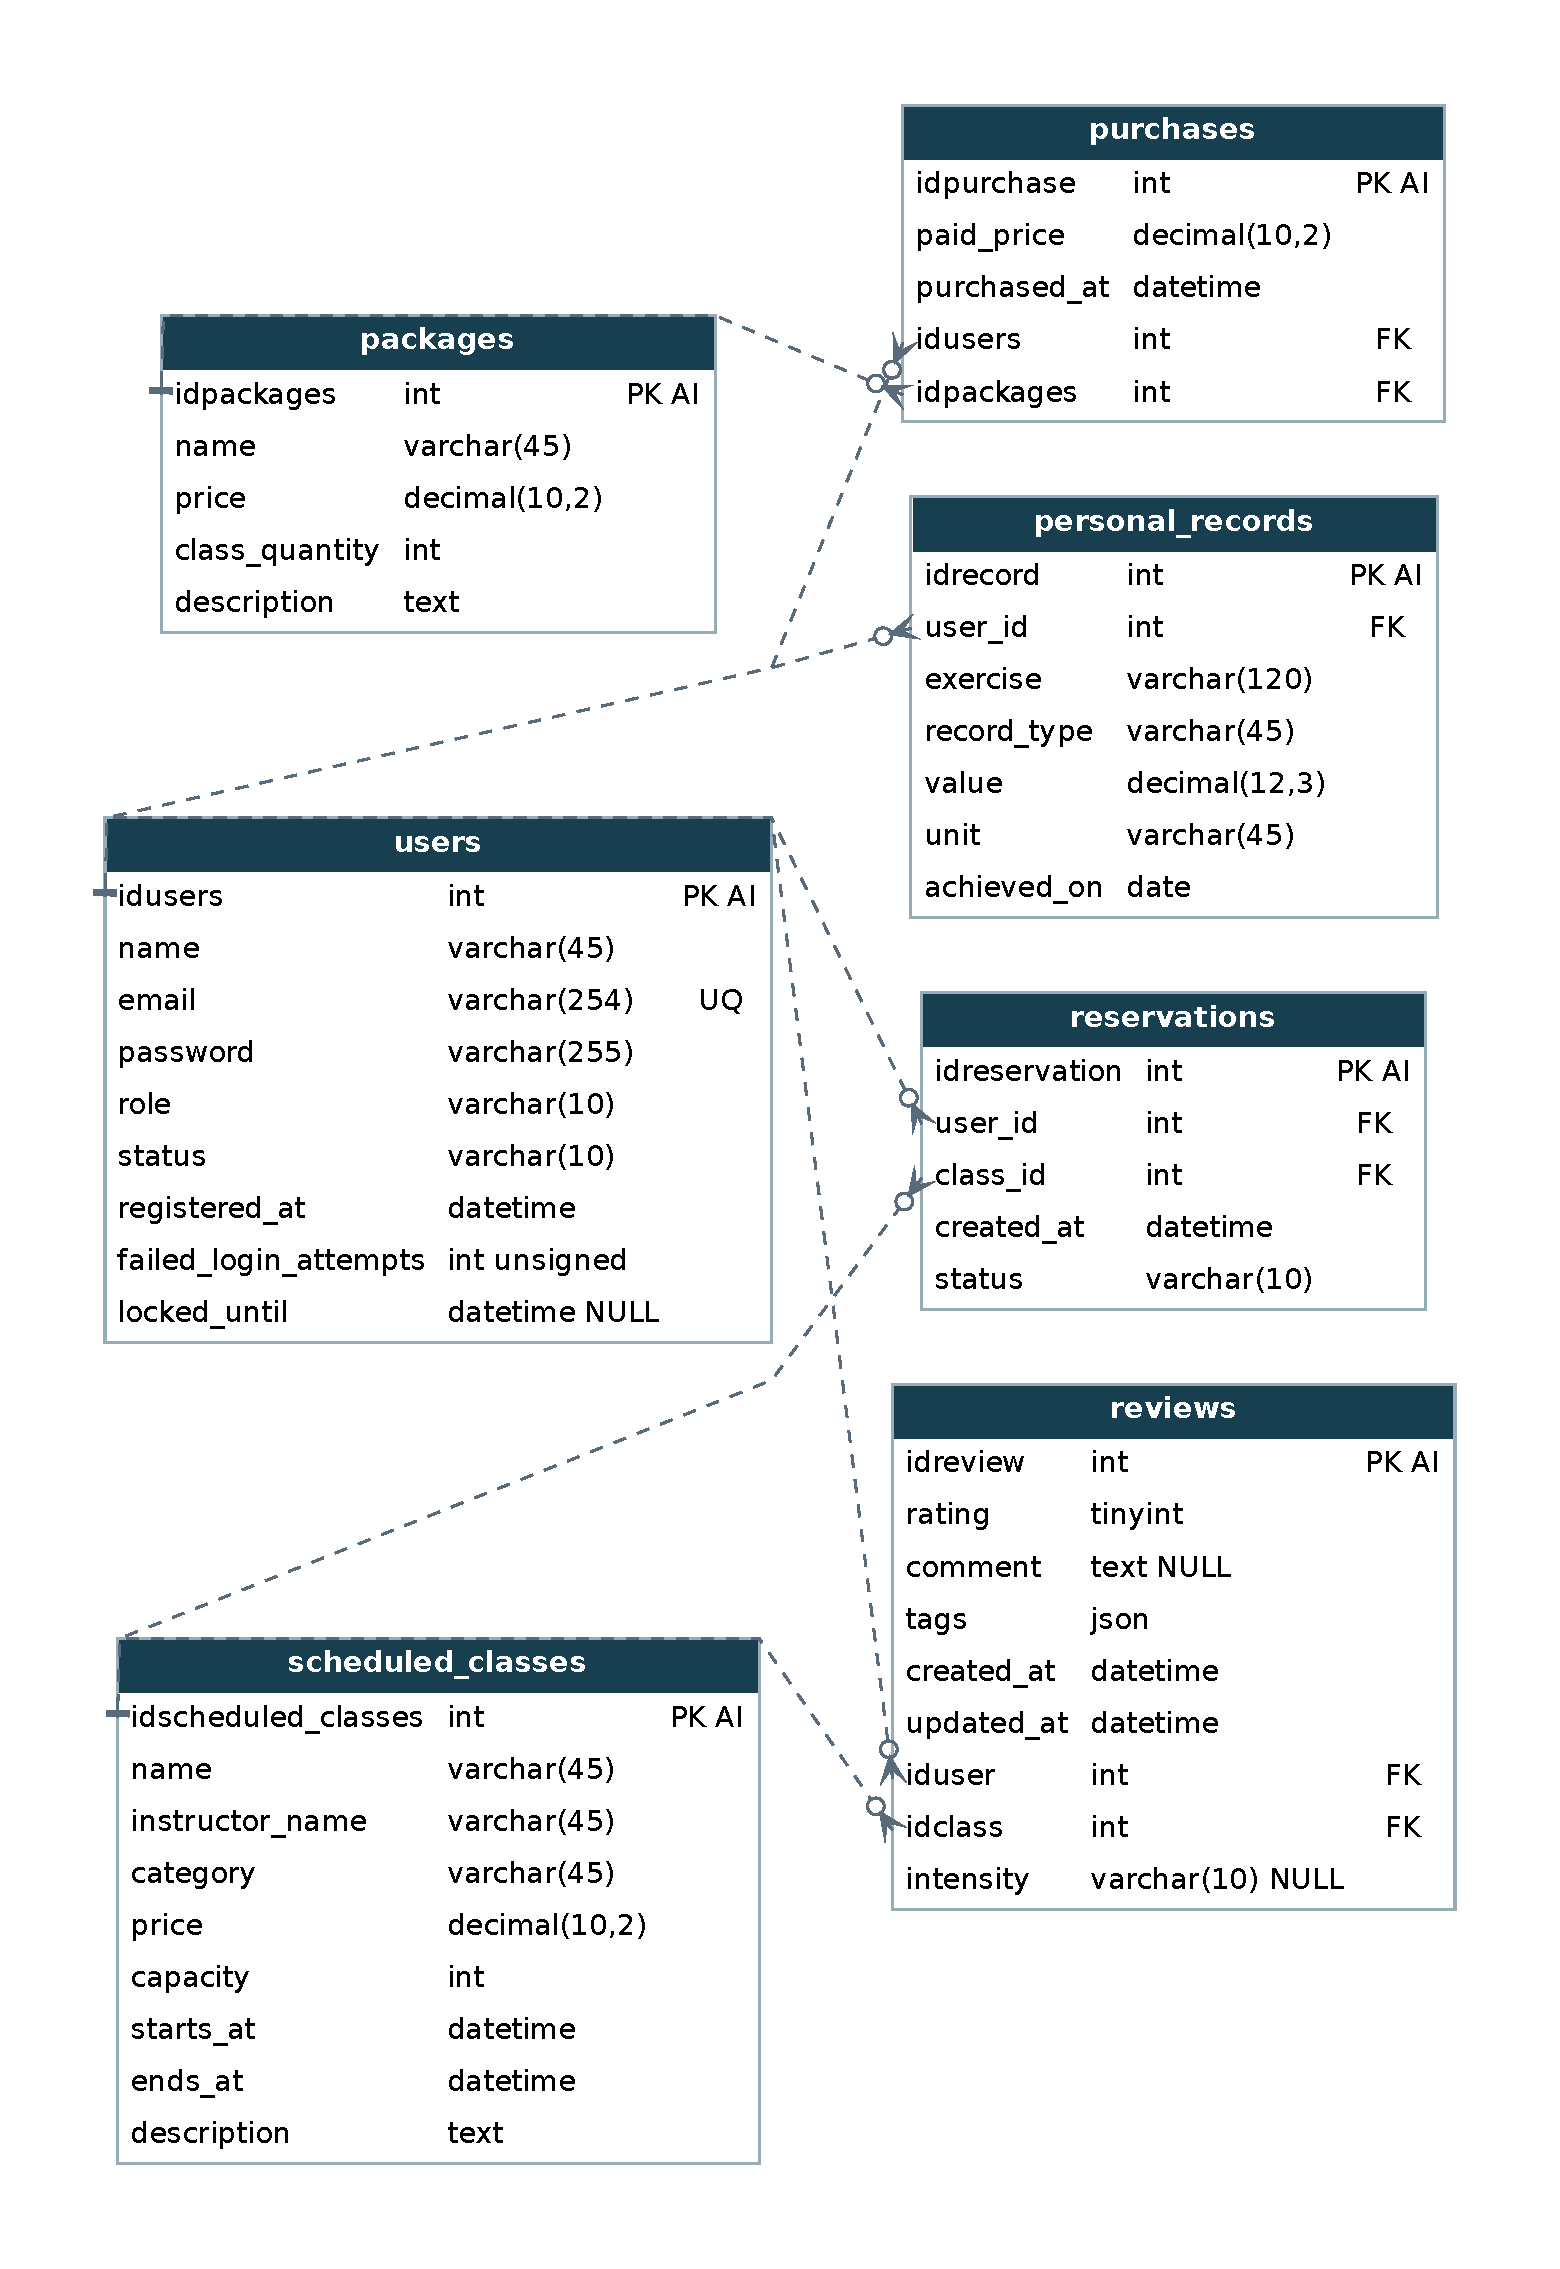
\includegraphics[width=\textwidth,height=.78\textheight,keepaspectratio]{figuras/modelo/modelo-fisico.pdf}
\caption{Modelo físico derivado de los metadatos reales de MySQL. El extremo simple indica un padre; el extremo de círculo y pata de cuervo indica cero o muchos hijos.}\label{fig:modelo-laura}
\end{figure*}

\section{Recursos REST y trazabilidad}\label{sec:rest-laura}
\subsection{Recursos, relaciones y métodos}
La API utiliza el prefijo \texttt{/api/v1}. Los nombres de ruta identifican recursos y los verbos HTTP expresan la operación. El contrato OpenAPI 3.0.3 describe parámetros, cuerpos y respuestas~\cite{openapi}. Hay 35 combinaciones de método y ruta; no son 35 tablas ni 35 recursos independientes.

Los identificadores de relaciones se envían como referencias: \texttt{packageId} para comprar y \texttt{classId} para reservar o reseñar. Las colecciones personales se anidan en el usuario, por ejemplo \texttt{/users/\{userId\}/reservations}. Las reseñas de una clase se consultan en \texttt{/classes/\{classId\}/reviews}. Se evita duplicar los datos de usuario, clase o paquete en las solicitudes.

\texttt{POST /sessions} crea una sesión lógica y devuelve el token; no existe una tabla de sesiones. \texttt{GET /reports/sales} y el recurso de progreso son consultas derivadas. La asistencia y el estado de una cuenta se representan con subrecursos que admiten \texttt{PATCH}.

\subsection{Operaciones disponibles}
Las Tablas~\ref{tab:operaciones-laura-1} y~\ref{tab:operaciones-laura-2} enumeran el contrato. Salvo registro e inicio de sesión, todas las operaciones exigen autenticación. El cliente consulta sus datos; el administrador puede consultar datos personales ajenos, pero no modificar una reseña o marca en nombre de su autor.
\begin{table*}[!t]\caption{Operaciones HTTP (1/2)}\label{tab:operaciones-laura-1}\centering\footnotesize
\begin{tabular}{p{.54\textwidth}p{.20\textwidth}p{.19\textwidth}}\toprule
Método y recurso & Acceso & Respuestas documentadas \\ \midrule
\texttt{POST /\allowbreak{}sessions} & Público & 201, 400, 401, 403, 423 \\
\texttt{POST /\allowbreak{}users} & Público & 201, 400, 409 \\
\texttt{GET /\allowbreak{}users} & Administrador & 200, 400, 401, 403 \\
\texttt{GET /\allowbreak{}users/\allowbreak{}\{id\}} & Propietario o admin & 200, 400, 401, 403, 404 \\
\texttt{PATCH /\allowbreak{}users/\allowbreak{}\{id\}/\allowbreak{}status} & Administrador & 200, 400, 401, 403, 404 \\
\texttt{GET /\allowbreak{}users/\allowbreak{}\{userId\}/\allowbreak{}purchases} & Propietario o admin & 200, 400, 401, 403, 404 \\
\texttt{GET /\allowbreak{}users/\allowbreak{}\{userId\}/\allowbreak{}reservations} & Propietario o admin & 200, 400, 401, 403, 404 \\
\texttt{GET /\allowbreak{}users/\allowbreak{}\{userId\}/\allowbreak{}personal-records} & Propietario o admin & 200, 400, 401, 403, 404 \\
\texttt{POST /\allowbreak{}users/\allowbreak{}\{userId\}/\allowbreak{}personal-records} & Cliente propietario & 201, 400, 401, 403 \\
\texttt{GET /\allowbreak{}users/\allowbreak{}\{userId\}/\allowbreak{}progress} & Propietario o admin & 200, 400, 401, 403, 404 \\
\texttt{GET /\allowbreak{}classes} & Autenticado & 200, 400, 401, 403 \\
\texttt{POST /\allowbreak{}classes} & Administrador & 201, 400, 401, 403 \\
\texttt{GET /\allowbreak{}classes/\allowbreak{}\{id\}} & Autenticado & 200, 400, 401, 403, 404 \\
\texttt{PATCH /\allowbreak{}classes/\allowbreak{}\{id\}} & Administrador & 200, 400, 401, 403, 404, 409 \\
\texttt{DELETE /\allowbreak{}classes/\allowbreak{}\{id\}} & Administrador & 204, 400, 401, 403, 404, 409 \\
\texttt{GET /\allowbreak{}classes/\allowbreak{}\{classId\}/\allowbreak{}reviews} & Autenticado & 200, 400, 401, 403, 404 \\
\texttt{GET /\allowbreak{}packages} & Autenticado & 200, 400, 401, 403 \\
\texttt{POST /\allowbreak{}packages} & Administrador & 201, 400, 401, 403 \\
\bottomrule\end{tabular}\end{table*}
\begin{table*}[!t]\caption{Operaciones HTTP (2/2)}\label{tab:operaciones-laura-2}\centering\footnotesize
\begin{tabular}{p{.54\textwidth}p{.20\textwidth}p{.19\textwidth}}\toprule
Método y recurso & Acceso & Respuestas documentadas \\ \midrule
\texttt{GET /\allowbreak{}packages/\allowbreak{}\{id\}} & Autenticado & 200, 400, 401, 403, 404 \\
\texttt{PATCH /\allowbreak{}packages/\allowbreak{}\{id\}} & Administrador & 200, 400, 401, 403, 404, 409 \\
\texttt{DELETE /\allowbreak{}packages/\allowbreak{}\{id\}} & Administrador & 204, 400, 401, 403, 404, 409 \\
\texttt{POST /\allowbreak{}purchases} & Cliente propietario & 201, 400, 401, 403, 404 \\
\texttt{GET /\allowbreak{}purchases} & Administrador & 200, 400, 401, 403 \\
\texttt{GET /\allowbreak{}purchases/\allowbreak{}\{id\}} & Propietario o admin & 200, 400, 401, 403, 404 \\
\texttt{POST /\allowbreak{}reservations} & Cliente propietario & 201, 400, 401, 403, 404, 409 \\
\texttt{GET /\allowbreak{}reservations/\allowbreak{}\{id\}} & Propietario o admin & 200, 400, 401, 403, 404 \\
\texttt{PATCH /\allowbreak{}reservations/\allowbreak{}\{id\}/\allowbreak{}attendance} & Administrador & 200, 400, 401, 403, 404, 409 \\
\texttt{POST /\allowbreak{}reviews} & Cliente propietario & 201, 400, 401, 403, 404, 409 \\
\texttt{GET /\allowbreak{}reviews/\allowbreak{}\{id\}} & Autenticado & 200, 400, 401, 403, 404 \\
\texttt{PATCH /\allowbreak{}reviews/\allowbreak{}\{id\}} & Cliente propietario & 200, 400, 401, 403, 404 \\
\texttt{DELETE /\allowbreak{}reviews/\allowbreak{}\{id\}} & Cliente propietario & 204, 400, 401, 403, 404 \\
\texttt{GET /\allowbreak{}personal-records/\allowbreak{}\{id\}} & Propietario o admin & 200, 400, 401, 403, 404 \\
\texttt{PATCH /\allowbreak{}personal-records/\allowbreak{}\{id\}} & Cliente propietario & 200, 400, 401, 403, 404 \\
\texttt{DELETE /\allowbreak{}personal-records/\allowbreak{}\{id\}} & Cliente propietario & 204, 400, 401, 403, 404 \\
\texttt{GET /\allowbreak{}reports/\allowbreak{}sales} & Administrador & 200, 400, 401, 403 \\
\bottomrule\end{tabular}\end{table*}
\subsection{Respuestas y operaciones excluidas}
Una creación devuelve \texttt{201} y la cabecera \texttt{Location}; una consulta o modificación, \texttt{200}; una eliminación correcta, \texttt{204}, sin cuerpo. Los datos se envuelven en \texttt{data}. Los errores se devuelven como \texttt{error.message}: \texttt{400} para entrada inválida, \texttt{401} para sesión ausente o inválida, \texttt{403} para permisos insuficientes, \texttt{404} para un recurso inexistente, \texttt{409} para un conflicto y \texttt{423} durante el bloqueo de cuenta.

No se ofrece eliminación de compras ni de reservas: representan hechos del historial. El usuario se desactiva en lugar de eliminarse. Los paquetes comprados quedan protegidos frente a modificación y eliminación. Las clases con reservas no se modifican; solo se eliminan clases futuras sin reservas. La asistencia confirmada no puede cambiarse a un resultado distinto. Estas decisiones protegen el historial y explican por qué no se fuerza un CRUD idéntico sobre todos los recursos.

\subsection{Trazabilidad funcional}
Las Tablas~\ref{tab:traza-laura-1} a~\ref{tab:traza-laura-3} conectan los 15 requerimientos con las historias, tablas y operaciones. Los nombres de Postman coinciden exactamente con la colección ejecutable de \texttt{evidence}. Una petición es evidencia de una parte del requisito; no prueba por sí sola toda su amplitud. RF-11 verifica autorización del backend: no constituye evidencia de un panel web implementado. Las comprobaciones adicionales de concurrencia y límites se describen en la sección de pruebas del informe general.
\begin{table*}[!t]\caption{Trazabilidad funcional (1/3)}\label{tab:traza-laura-1}\centering\scriptsize\setlength{\tabcolsep}{4pt}
\begin{tabular}{p{.09\textwidth}p{.20\textwidth}p{.25\textwidth}p{.39\textwidth}}\toprule
RF / historia & Tablas & Operaciones & Peticiones de Postman \\ \midrule
RF-01 / CO-1 & \texttt{users} & \texttt{POST /\allowbreak{}users} & POST /\allowbreak{}users - register client - success (201); POST /\allowbreak{}users - invalid email - error (400) \\
RF-02 / CO-2 & \texttt{users} & \texttt{POST /\allowbreak{}sessions} & POST /\allowbreak{}sessions - client login - success (201); POST /\allowbreak{}sessions - unknown email - error (401) \\
RF-03 / CO-3, CO-4 & \texttt{scheduled\_\allowbreak{}classes} & \texttt{GET /\allowbreak{}classes}; \texttt{GET /\allowbreak{}classes/\allowbreak{}\{id\}} & GET /\allowbreak{}classes - success (200); GET /\allowbreak{}classes/\allowbreak{}\{id\} - success (200); GET /\allowbreak{}classes/\allowbreak{}\{id\} - missing class - error (404) \\
RF-04 / CO-5 & \texttt{users}, \texttt{packages}, \texttt{purchases} & \texttt{POST /\allowbreak{}purchases} & POST /\allowbreak{}purchases - success (201); POST /\allowbreak{}purchases - client sends price - error (400) \\
RF-05 / CO-6 & \texttt{users}, \texttt{scheduled\_\allowbreak{}classes}, \texttt{reservations} & \texttt{POST /\allowbreak{}reservations} & POST /\allowbreak{}reservations - success (201); POST /\allowbreak{}reservations - duplicate - error (409) \\
\bottomrule\end{tabular}\end{table*}
\begin{table*}[!t]\caption{Trazabilidad funcional (2/3)}\label{tab:traza-laura-2}\centering\scriptsize\setlength{\tabcolsep}{4pt}
\begin{tabular}{p{.09\textwidth}p{.20\textwidth}p{.25\textwidth}p{.39\textwidth}}\toprule
RF / historia & Tablas & Operaciones & Peticiones de Postman \\ \midrule
RF-06 / CO-7, CO-8 & \texttt{reservations}, \texttt{scheduled\_\allowbreak{}classes} & \texttt{GET /\allowbreak{}users/\allowbreak{}\{userId\}/\allowbreak{}reservations}; \texttt{PATCH /\allowbreak{}reservations/\allowbreak{}\{id\}/\allowbreak{}attendance} & GET /\allowbreak{}users/\allowbreak{}\{userId\}/\allowbreak{}reservations - success (200); PATCH /\allowbreak{}reservations/\allowbreak{}\{id\}/\allowbreak{}attendance - finished class - success (200); PATCH /\allowbreak{}reservations/\allowbreak{}\{id\}/\allowbreak{}attendance - class not ended - error (409) \\
RF-07 / CO-9, CO-10 & \texttt{reviews}, \texttt{reservations}, \texttt{scheduled\_\allowbreak{}classes} & \texttt{POST /\allowbreak{}reviews}; \texttt{PATCH /\allowbreak{}reviews/\allowbreak{}\{id\}}; \texttt{DELETE /\allowbreak{}reviews/\allowbreak{}\{id\}} & POST /\allowbreak{}reviews - attended class - success (201); POST /\allowbreak{}reviews - class not attended - error (409); PATCH /\allowbreak{}reviews/\allowbreak{}\{id\} - success (200); DELETE /\allowbreak{}reviews/\allowbreak{}\{id\} - success (204) \\
RF-08 / CO-11 & \texttt{reservations}, \texttt{scheduled\_\allowbreak{}classes} & \texttt{GET /\allowbreak{}users/\allowbreak{}\{userId\}/\allowbreak{}progress} & GET /\allowbreak{}users/\allowbreak{}\{userId\}/\allowbreak{}progress - success (200); GET /\allowbreak{}users/\allowbreak{}\{userId\}/\allowbreak{}progress - other user - error (403) \\
RF-09 / CO-12 & \texttt{reservations}, \texttt{scheduled\_\allowbreak{}classes} & \texttt{GET /\allowbreak{}users/\allowbreak{}\{userId\}/\allowbreak{}progress} & GET /\allowbreak{}users/\allowbreak{}\{userId\}/\allowbreak{}progress - success (200); GET /\allowbreak{}users/\allowbreak{}\{userId\}/\allowbreak{}progress - other user - error (403) \\
RF-10 / CO-13 & \texttt{users}, \texttt{personal\_\allowbreak{}records} & \texttt{POST /\allowbreak{}users/\allowbreak{}\{userId\}/\allowbreak{}personal-records}; \texttt{GET /\allowbreak{}users/\allowbreak{}\{userId\}/\allowbreak{}personal-records}; \texttt{PATCH /\allowbreak{}personal-records/\allowbreak{}\{id\}}; \texttt{DELETE /\allowbreak{}personal-records/\allowbreak{}\{id\}} & POST /\allowbreak{}users/\allowbreak{}\{userId\}/\allowbreak{}personal-records - success (201); GET /\allowbreak{}users/\allowbreak{}\{userId\}/\allowbreak{}personal-records - other user - error (403); PATCH /\allowbreak{}personal-records/\allowbreak{}\{id\} - success (200); DELETE /\allowbreak{}personal-records/\allowbreak{}\{id\} - success (204) \\
\bottomrule\end{tabular}\end{table*}
\begin{table*}[!t]\caption{Trazabilidad funcional (3/3)}\label{tab:traza-laura-3}\centering\scriptsize\setlength{\tabcolsep}{4pt}
\begin{tabular}{p{.09\textwidth}p{.20\textwidth}p{.25\textwidth}p{.39\textwidth}}\toprule
RF / historia & Tablas & Operaciones & Peticiones de Postman \\ \midrule
RF-11 / AO-1 & \texttt{users} & \texttt{POST /\allowbreak{}sessions}; \texttt{GET /\allowbreak{}users} & POST /\allowbreak{}sessions - admin login - success (201); GET /\allowbreak{}users - admin - success (200); GET /\allowbreak{}users - client role - error (403) \\
RF-12 / AO-2 & \texttt{scheduled\_\allowbreak{}classes} & \texttt{POST /\allowbreak{}classes}; \texttt{PATCH /\allowbreak{}classes/\allowbreak{}\{id\}}; \texttt{DELETE /\allowbreak{}classes/\allowbreak{}\{id\}} & POST /\allowbreak{}classes - success (201); POST /\allowbreak{}classes - client role - error (403); PATCH /\allowbreak{}classes/\allowbreak{}\{id\} - success (200); DELETE /\allowbreak{}classes/\allowbreak{}\{id\} - success (204) \\
RF-13 / AO-3 & \texttt{purchases} & \texttt{GET /\allowbreak{}reports/\allowbreak{}sales} & GET /\allowbreak{}reports/\allowbreak{}sales - admin - success (200); GET /\allowbreak{}reports/\allowbreak{}sales - invalid date - error (400) \\
RF-14 / AO-4 & \texttt{purchases}, \texttt{users}, \texttt{packages} & \texttt{GET /\allowbreak{}purchases}; \texttt{GET /\allowbreak{}purchases/\allowbreak{}\{id\}} & GET /\allowbreak{}purchases - admin - success (200); GET /\allowbreak{}purchases - client role - error (403) \\
RF-15 / AO-5 & \texttt{users} & \texttt{GET /\allowbreak{}users}; \texttt{PATCH /\allowbreak{}users/\allowbreak{}\{id\}/\allowbreak{}status} & GET /\allowbreak{}users - admin - success (200); PATCH /\allowbreak{}users/\allowbreak{}\{id\}/\allowbreak{}status - deactivate - success (200); PATCH /\allowbreak{}users/\allowbreak{}\{id\}/\allowbreak{}status - invalid status - error (400) \\
\bottomrule\end{tabular}\end{table*}

\section{Arquitectura de la API}\label{sec:arquitectura-laura}
\subsection{Separación de responsabilidades}
La organización por capas evita que una ruta mezcle autorización, reglas de negocio y consultas SQL. Express permite asociar rutas y middleware con los métodos HTTP~\cite{express}. La Fig.~\ref{fig:arquitectura-laura} resume la dirección principal de las dependencias.
\begin{figure}[!t]\centering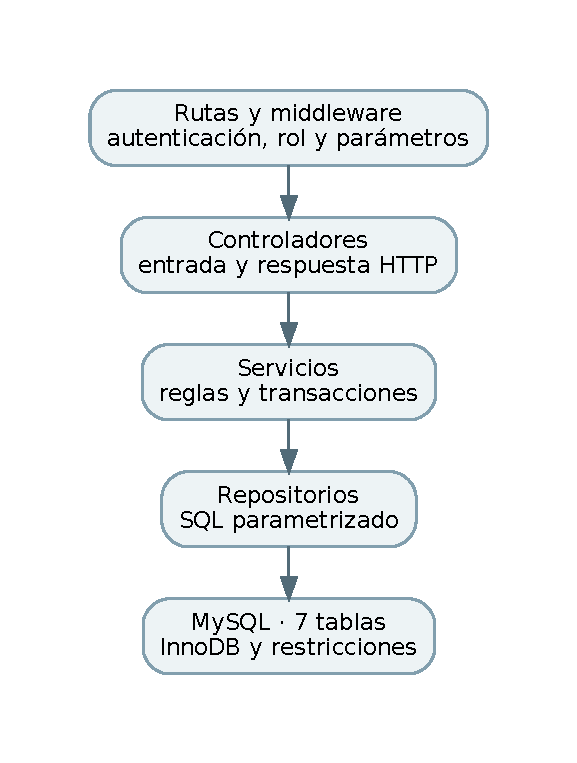
\includegraphics[width=.88\columnwidth,height=.42\textheight,keepaspectratio]{figuras/modelo/arquitectura.pdf}\caption{Capas de la API y persistencia.}\label{fig:arquitectura-laura}\end{figure}

\texttt{routes} declara recursos, métodos y controles de acceso. \texttt{controllers} convierte parámetros HTTP y selecciona respuestas. \texttt{services} aplica las reglas del gimnasio: cupos, horarios, propiedad, asistencia y protección del historial. \texttt{repositories} contiene SQL parametrizado y los alias de salida. \texttt{config} concentra conexión y variables de entorno; \texttt{utils} reúne validaciones y fechas comunes.

\subsection{Controles comunes}
El middleware valida el JWT y consulta la cuenta actual: un token existente no permite usar una cuenta desactivada. Los controles de rol y propiedad se combinan; conocer un identificador no concede acceso. El registro público asigna el rol \texttt{client} y rechaza un campo de rol enviado por el solicitante. Las credenciales y tokens se excluyen de las respuestas de perfil y se ocultan en las evidencias.

El manejador central de errores convierte conflictos y errores esperables en respuestas uniformes. Una excepción no controlada produce una respuesta genérica; los detalles SQL no se exponen al cliente. Esto mantiene el formato HTTP sin repetir el mismo manejo en cada controlador.

\subsection{Persistencia y concurrencia}
\texttt{database.js} administra el pool de conexiones y fija UTC en las operaciones. Los servicios que necesitan atomicidad reciben una conexión transaccional y la pasan al repositorio. Una reserva bloquea la fila de la clase antes de contar cupos: la lectura y la inserción pertenecen a la misma transacción. Las restricciones de unicidad y de referencia agregan protección a las validaciones de aplicación.

No se permite que el cliente escriba SQL ni determine el precio pagado. La configuración se obtiene del entorno; \texttt{.env.example} documenta sus nombres sin guardar credenciales reales. La documentación interactiva y el contrato se sirven desde la aplicación en \texttt{/docs} y \texttt{/openapi.json}.

\section{Implementación}\label{sec:implementacion-laura}
\subsection{Preparación y compatibilidad del esquema}
\texttt{database/schema.sql} crea las siete tablas con claves primarias autoincrementales, claves foráneas, valores predeterminados y restricciones. \texttt{db:setup} prepara una base nueva y comprueba su compatibilidad. \texttt{db:seed} crea el administrador y paquetes de demostración; \texttt{db:demo} prepara un cliente y una reserva de una clase terminada para ejercitar la asistencia.

El arranque comprueba la conexión antes de escuchar peticiones. Se amplió \texttt{checkSchema} para detectar columnas faltantes, identificadores sin autoincremento y columnas heredadas obligatorias sin valor predeterminado. Evita anunciar una API lista cuando las inserciones fallarán por esas diferencias. No modifica ni migra datos de una base existente, y no certifica todos los tipos o restricciones; una migración requiere comparar el esquema completo.

\subsection{Compra y protección del precio}
En \texttt{purchase-service.js}, el cuerpo solo admite \texttt{packageId}. El usuario comprador se obtiene de la sesión y el precio del paquete se lee dentro de la transacción. El fragmento siguiente pertenece al servicio real; no permite sustituir el precio con un valor enviado por el comprador.
\begin{lstlisting}[caption={Precio de compra elegido por el servidor.}]
return transaction(async (connection) => {
  const item = found(await packages.findById(
    packageId, connection, true), 'Package');
  return repository.create(user.id, packageId,
    item.price, connection);
});
\end{lstlisting}

\subsection{Reserva, asistencia y reseña}
\texttt{reservation-service.js} verifica horario, duplicidad y cupo antes de insertar. El bloqueo de la clase mantiene la decisión de cupo dentro de la transacción. El siguiente fragmento aplica el rechazo cuando no quedan plazas.
\begin{lstlisting}[caption={Control de cupo en la transacción de reserva.}]
const total = await classes.reservationCount(
  classId, connection);
if (total >= item.capacity) {
  fail(409, 'The class is full');
}
return repository.create(user.id,
  classId, connection);
\end{lstlisting}
El administrador registra \texttt{attended} o \texttt{no\_show} después de terminar la clase. \texttt{review-service.js} exige la reserva del usuario con estado \texttt{attended}; rechaza una clase no asistida y una reseña duplicada. La calificación es obligatoria. Comentario e intensidad pueden omitirse; las etiquetas omitidas se convierten en un arreglo vacío. Eliminar una reseña conserva la reserva y la asistencia.

\subsection{Progreso y marcas personales}
\texttt{progress-service.js} usa únicamente reservas asistidas, agrupa por categoría y deduplica semanas para calcular la racha. La semana inicia el lunes y la fecha de negocio usa \texttt{America/Bogota}; una clase se asigna a la semana de su inicio. La racha puede continuar desde la semana anterior si la semana actual aún no tiene asistencia.

\texttt{record-service.js} conserva ejercicio, tipo, valor, unidad y fecha. Rechaza valores no positivos y fechas futuras; el propietario puede crear, modificar o eliminar su marca. La API entrega el historial registrado, sin atribuirle un cálculo automático de máximos ni comparaciones entre unidades diferentes.

\subsection{Lectura del código y alcance}
Los fragmentos muestran las decisiones que conectan el modelo con las reglas. La ejecución automática, las mediciones y las respuestas capturadas pertenecen a la sección de pruebas del informe general. El backend permite construir las vistas del cliente y del administrador, pero la existencia de los endpoints no equivale a una interfaz implementada.

\balance
\bibliographystyle{IEEEtran}
\bibliography{referencias-laura}
\end{document}
